\documentclass[a4paper,12pt]{report} %размер бумаги устанавливаем А4, шрифт 14пунктов
\usepackage[T2A]{fontenc}
\usepackage[utf8]{inputenc}%включаем свою кодировку: koi8-r или utf8 в UNIX, cp1251 в Windows
\usepackage[english,russian]{babel}%используем русский и английский языки с переносами
\usepackage{amssymb,amsfonts,amsmath,mathtext,cite,enumerate,float,caption} %подключаем нужные пакеты расширений
\usepackage[dvips]{graphicx} %хотим вставлять в диплом рисунки?
\graphicspath{{images/}}%путь к рисункам

\makeatletter
\renewcommand{\@biblabel}[1]{#1.} % Заменяем библиографию с квадратных скобок на точку:
\makeatother

\usepackage{geometry} % Меняем поля страницы
\geometry{left=2cm}% левое поле
\geometry{right=1.5cm}% правое поле
\geometry{top=1cm}% верхнее поле
\geometry{bottom=2cm}% нижнее поле

\setlength{\parindent}{1cm} % настройка красной строки

\captionsetup[table]{singlelinecheck=false,justification=raggedleft} %выравнивание по правому краю заголовков таблиц

\renewcommand{\theenumi}{\arabic{enumi}}% Меняем везде перечисления на цифра.цифра
\renewcommand{\labelenumi}{\arabic{enumi}}% Меняем везде перечисления на цифра.цифра
\renewcommand{\theenumii}{.\arabic{enumii}}% Меняем везде перечисления на цифра.цифра
\renewcommand{\labelenumii}{\arabic{enumi}.\arabic{enumii}.}% Меняем везде перечисления на цифра.цифра
\renewcommand{\theenumiii}{.\arabic{enumiii}}% Меняем везде перечисления на цифра.цифра
\renewcommand{\labelenumiii}{\arabic{enumi}.\arabic{enumii}.\arabic{enumiii}.}% Меняем везде перечисления на цифра.цифра


\begin{document}
\begin{titlepage}
    \newpage
    
    \begin{center}
    ПРАВИТЕЛЬСТВО РОССИЙСКОЙ ФЕДЕРАЦИИ \\
    \vspace{1em}
    ФЕДЕРАЛЬНОЕ  ГОСУДАРСТВЕННОЕ АВТОНОМНОЕ \\
    ОБРАЗОВАТЕЛЬНОЕ УЧРЕЖДЕНИЕ ВЫСШЕГО ОБРАЗОВАНИЯ \\
    <<НАЦИОНАЛЬНЫЙ ИССЛЕДОВАТЕЛЬСКИЙ УНИВЕРСИТЕТ \\
    <<ВЫСШАЯ ШКОЛА ЭКОНОМИК>> \\
    \vspace{2em}
    \textbf{Московский институт электроники и математики им. А.Н. Тихонова}\\
    \vspace{6em}
    Степушин Кирилл Алексеевич\\
    \vspace{3em}
    \textbf{РАЗРАБОТКА ОТЛАДЧИКА С МОНИТОРИНГОМ ЭНЕРГОПОТРЕБЛЕНИЯ}\\
    \vspace{6em}
    Выпускная квалификационная работа -- магистерская диссертация\\ 
    по направлению 11.04.02 «Инфокоммуникационные технологии и системы связи»\\
    студента образовательной программы магистратуры\\
    «Интернет вещей и киберфизические системы»
    \end{center}

    \vspace{6em}

    \begin{flushleft}
    Студент \hfill Научный руководитель\\
    \hfill приглашенный преподаватель\\
    \vspace{1em}
    \rule{5cm}{0.005cm} \hfill \rule{5cm}{0.01cm}\\
    \hfill И.О.Фамилия

    \vspace{1em}

    Рецензент \hfill Консультант\\
    к.т.н., доцент \hfill приглашенный преподаватель\\
    \vspace{1em}
    \rule{5cm}{0.005cm} \hfill \rule{5cm}{0.01cm}\\
    И.О.Фамилия \hfill И.О.Фамилия
    \end{flushleft}
    
    \vspace{\fill}
    
    \begin{center}
    Москва 2024
    \end{center}
    
    \end{titlepage}%титульный лист
\tableofcontents %оглавление, которое генерируется автоматически

\chapter*{Введение}
\addcontentsline{toc}{chapter}{Введение}
\hspace{1cm} Независимо от стараний разработчика или сложности проекта, большая часть времени разработки
будет потрачена на то, чтобы убедиться, что устройство работает правильно, или -- что наиболее
вероятно -- разобраться, почему устройство работает не так, как ожидалось. Отладчик -- самый мощный 
инструмент в наборе инструментов разработчика, позволяющий напрямую взаимодействовать с процессором,
задавать точки останова, пошагово управлять потоком выполнения инструкций и проверять  значения
регистров. \cite{Lakamera:embed}

Для устройств <<интернета вещей>> очень важно знать и отслеживать энергопотребление,
ведь обычно такие устройства питаются от батарейки и каждое ненужное действие уменьшит
срок службы. Мониторинг энергопотребления позволяет понять энергоэффективность каждого сеанса связи,
что позволит выбрать наиболее подходящий интерфейс и протокол передачи данных.

Об актуальности возможности мониторинга энергопотребления для отладчика говорит количество 
измерительных устройств на рынке. Характеристики основных из них приведены в таблице 
\ref{comparemeasdevices}.

\begin{table}[H]
    \caption{Сравнение характеристик измерительных устройств}
    \label{comparemeasdevices}   
    \begin{center}
    \begin{tabular}{|c|c|c|c|c|}
    \hline
  Устройство & Joulescope & Otii Arc & NanoRanger & Current Ranger \\ \hline
    Диапазон тока & от -1 А до 3 А & от 0 до 2,5 А & от 1 нА до 800 мА & от -1,65 А до 3 А \\ \hline
    Разрешение & 1 нА & десятки нА & до 10 пА & до 1 пА  \\ \hline
    Погрешность & до 0,3\% & до 0,1\% & до 0,3\% & до 0,1\% \\ \hline
    Цена & 800 \$ & 700 \$ & 220 \$ & 120 \$  \\ \hline
    \end{tabular}
    \end{center}
\end{table} 

Так же о высокой потребности в устройстве говорит большое количество существующих отладчиков с 
мониторингом энергопотребления от различных производителей микроконтроллеров, например STLINK-V3 
\cite{STLINKV3} и Power Profiler Kit II \cite{Power Profiler Kit}, так и от сторонних компаний, например 
Energymon.

Потребность в таком отладчике также имеется у MIEM IoT-LAB для реализации возможности удаленного 
мониторинга энергопотребления, как как это сделано в оригинале у FIT IoT-LAB, а так же улучшение 
французского решения в сторону замены аппаратной реализации с PaspBerry на микроконтроллер и повышения 
точности и качества мониторинга потребляемой мощности у отлаживаемых устройств. \cite{FITIoT}.

Определяя требования к диапазонам измеряемого тока, стоит учитывать различные IoT-устройства. Грубую оценку
можно составить на примере Wi-Fi решений и сотовых модемов, которые в <<пике>> передачи данных могут 
иметь потребление в районе одного ампера, а в спящем режиме потребляют порядка единиц мкА.

%ссылку на инфу

Перед проектированием отладчика с возможностью мониторинга энергопотребления IoT-устройств
следует определиться с требованиями, предъявляемыми к отладчику. 
Для этого в качестве примера рассмотрим <<усредненный>> паттерн поведения устройства с BLE, одной
из самых популярных технологий беспроводной передачи данных интернета вещей, 
у которого с периодичностью в несколько десятков мс повторяется такой цикл: спящий режим 
с токопотреблением единицы мкА, далее устройство просыпается, в этот момент
энерго потребление составляет единицы мА, время просыпания -- десятки мкс, далее происходит
сеанс связи, который начинается с передачи, с токопотреблением примерно десятки мА 
и длительностью передачи <<пустого>> пакета величиной 27 байт около 200 мкс, и продолжается 
ожиданием ответа длительностью в среднем 150 мкс, после сеанс связи завершается приемом,
при котором токопотребление составляет единицы-десятки мА длительностью 200 мкс.

Зная ориентировочные диапазоны измеряемых токов, можно грубо промоделировать данный паттерн 
поведения BLE-устройства в LTSpice, чтобы оценить необходимую полосу пропускания отладчика. 
Моделируемая схема представлена на рисунке \ref{ris:LTSpiceScheme}, результаты моделирования 
представлены на рисунках \ref{ris:LTSpice0_01} - \ref{ris:LTSpice100} и имеют больше 
демонстрационно-оценочный характер.

\begin{figure}[H]
  \centering
  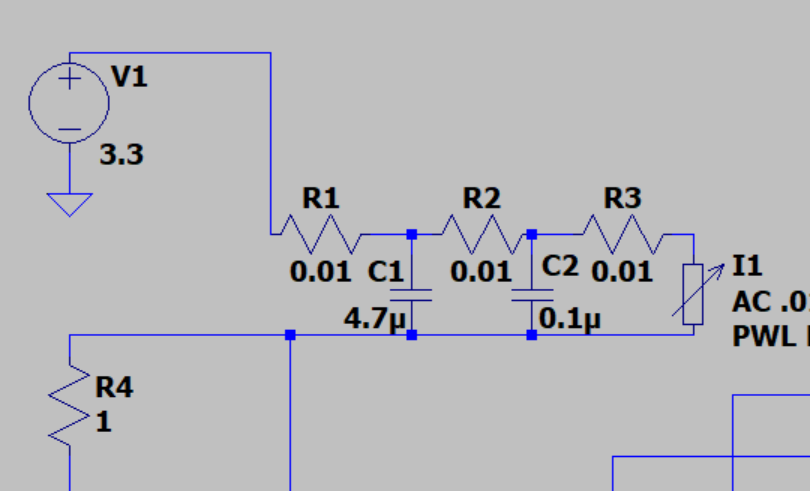
\includegraphics[scale = 0.5]{LPSpice scheme.png}
  \caption{Моделируемая схема}
  \label{ris:LTSpiceScheme}
\end{figure}

\begin{figure}[H]
  \centering
  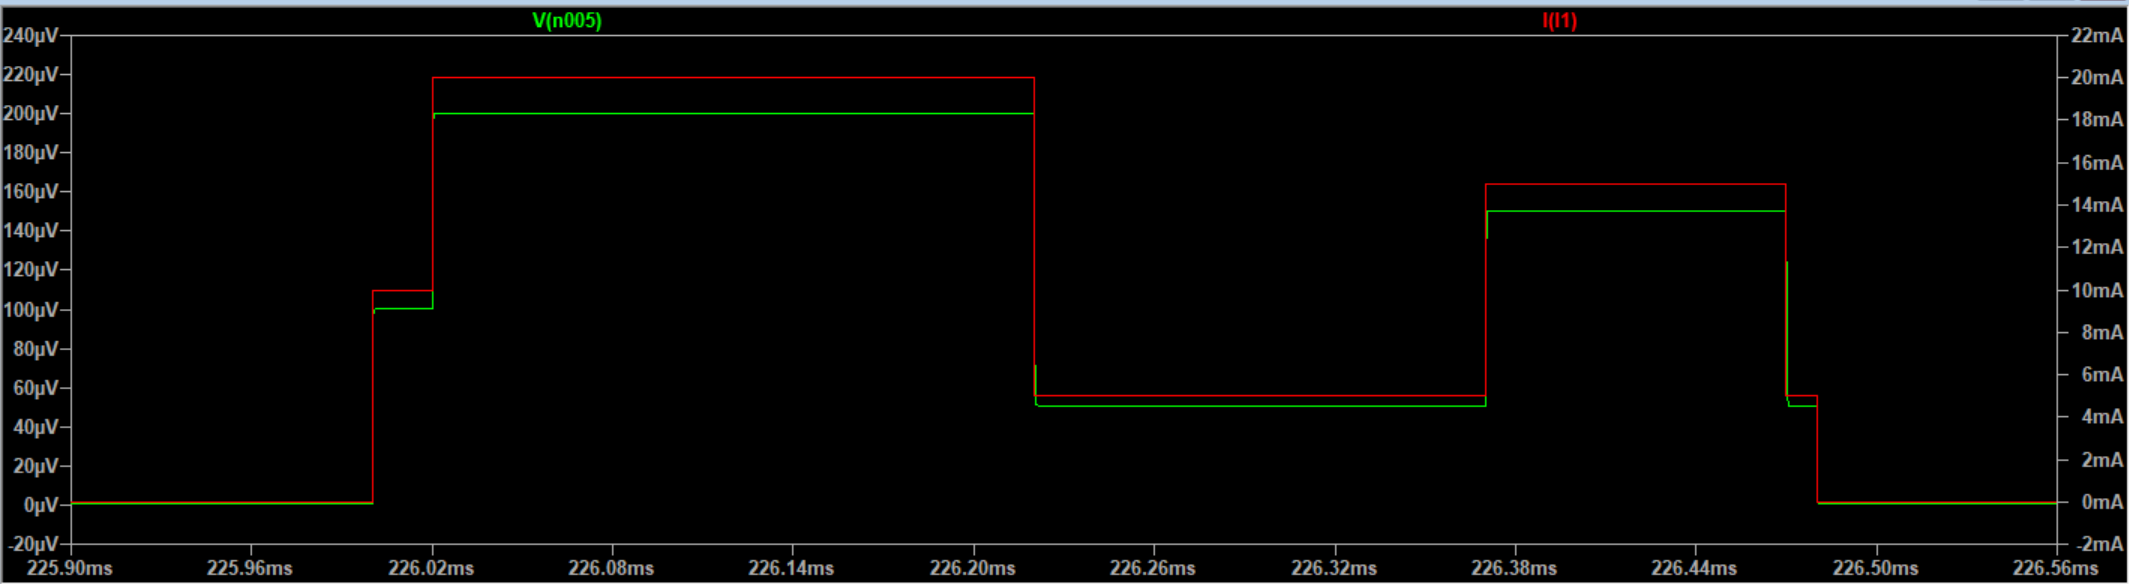
\includegraphics[scale = 0.3]{LTSpice0_01.png}
  \caption{Результаты моделирования амперного диапазона }
  \label{ris:LTSpice0_01}
\end{figure}

Резисторы R1 -- R3 моделируют сопротивления проводников на печатной плате, конденсаторы C1 -- C2 фильтрующие 
по питанию, I1 -- источник тока, моделирующий вышеописанный паттерн поведения BLE-устройства,
R4 - шунт, для амперного диапазона, который равен 0,01 Ом (в дальнейшем в ходе дипломной работы уточняется). 
Красная линия -- входной сигнал, моделирующий потребление отлаживаемого устройства, 
зеленная -- падение напряжения на измеряемом шунте. 

\begin{figure}[H]
  \centering
  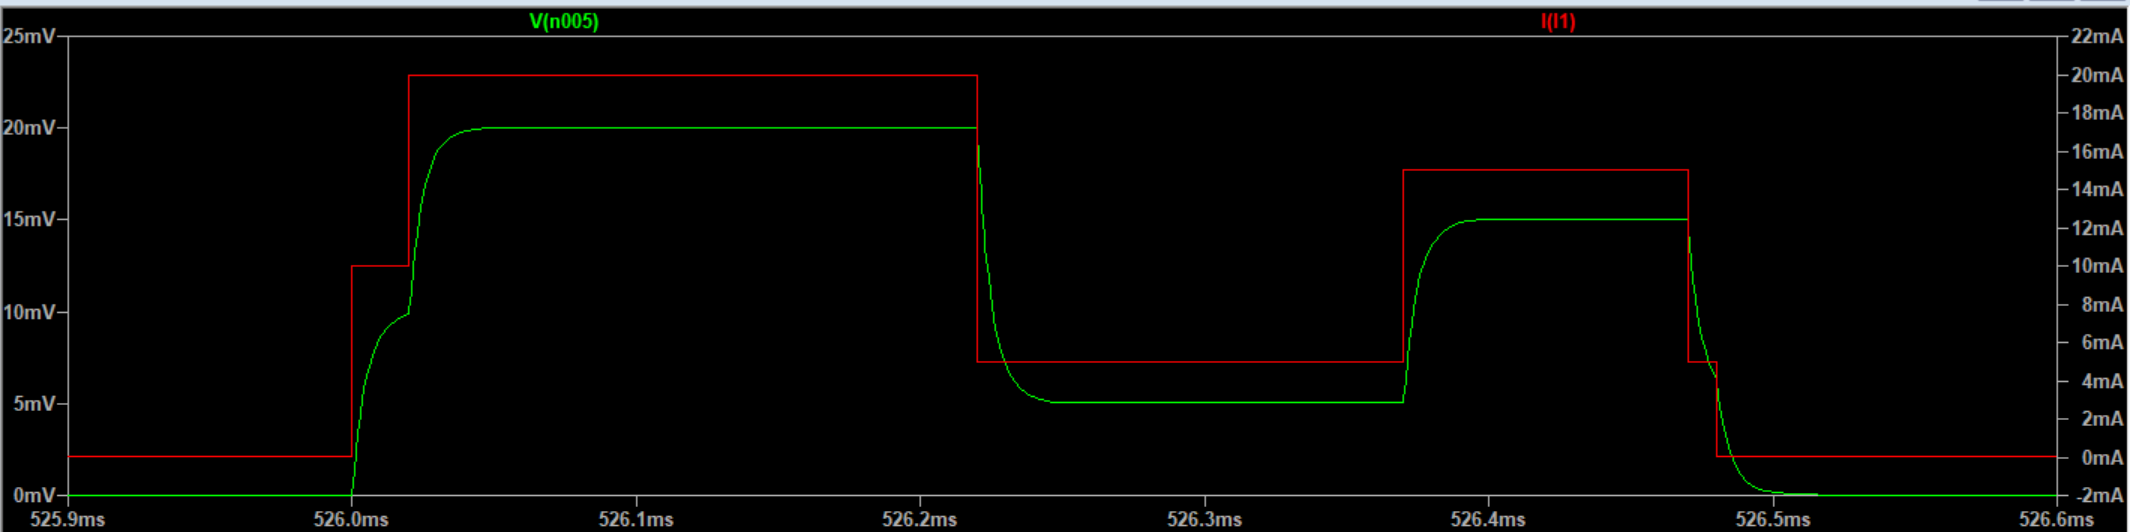
\includegraphics[scale = 0.3]{LTSpice_1.png}
  \caption{Результаты моделирования миллиамперного диапазона }
  \label{ris:LTSpice_1}
\end{figure}

Здесь шунт R4 равен 1 Ом, диапазон -- миллиамперный. 

\begin{figure}[H]
  \centering
  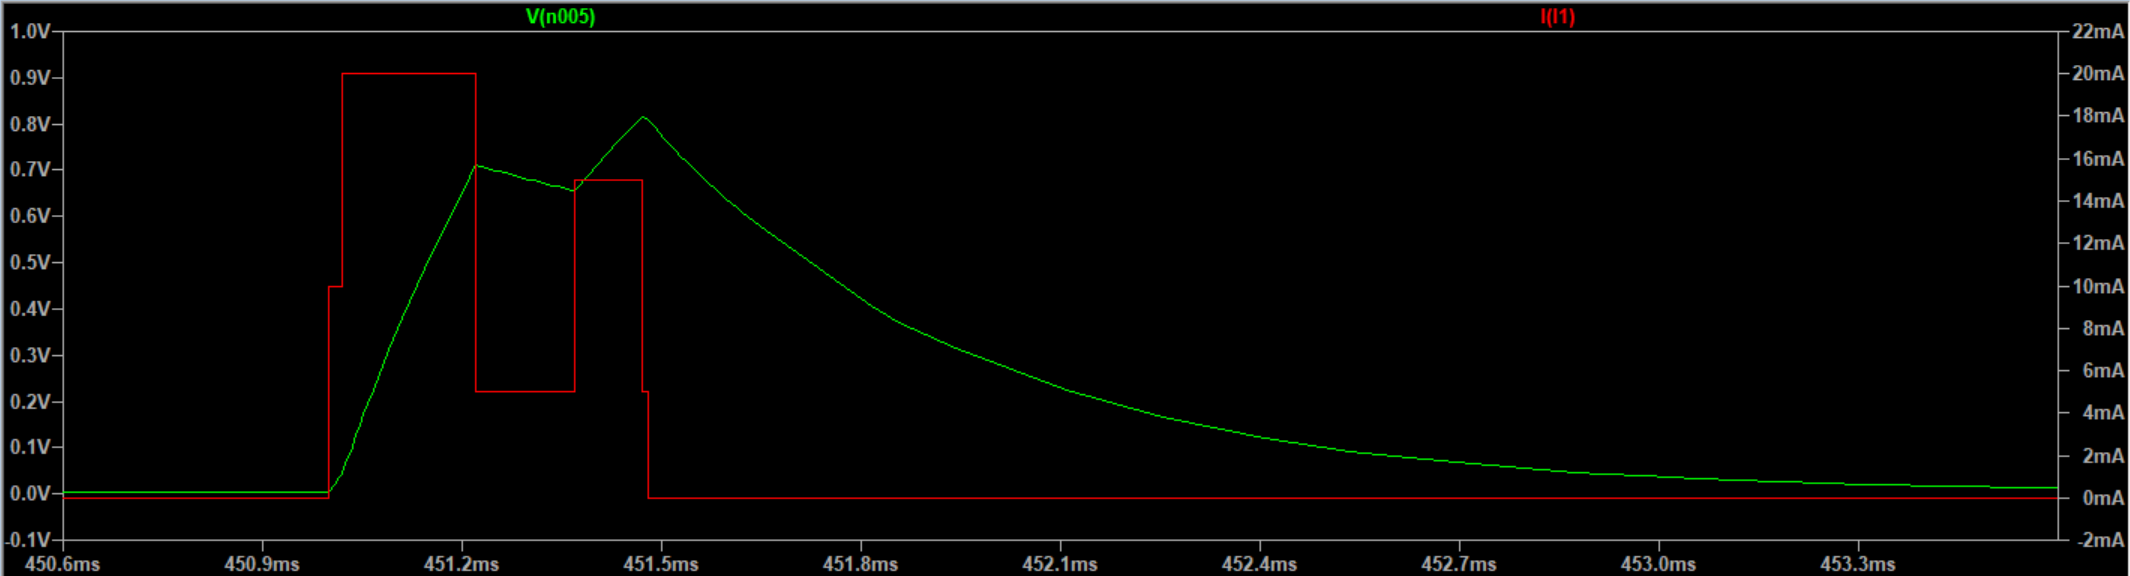
\includegraphics[scale = 0.3]{LTspice100.png}
  \caption{Результаты моделирования микроамперного диапазона }
  \label{ris:LTSpice100}
\end{figure}

А вот моделирование микроамперного диапазона, который можно считать основным измерительным диапазоном для 
IoT-устройств с малым энергопотреблением, показывает, что из-за получившегося из R1 -- R3 и C1 -- C2 RC-фильтра,
уменьшение полосы пропускания на порядки до, примерно, значения в  15 кГц, что определяет требование 
к полосе пропускания.

Так как разрабатываемое устройство является отладчиком, то для <<общения>> с отлаживаемым устройством 
в отладчике должны быть реализованы стандартные для этих целей интерфейсы, такие как UART и отладочные 
SWD/JTAG, что подразумевает под собой наличие удобных, распространенных разъемов. Так же из-за планируемого 
использования в MIEM IoT-LAB, отладчик должен уметь общаться с <<сервером>> по Ethernet, что, по сути,
является требованием заказчика, обусловленное потребностью в возможности гибкого размещения лаборатории на 
территории МИЭМа.  

Для обеспечения конкурентноспособности отладчика, остальные характеристики можно определить 
из таблицы \ref{comparemeasdevices}, а так же из анализа типичной используемой элементной базы.

Резюмируя вышесказанное, можно ориентироваться на следующие требования к разрабатываемому 
устройству:
\begin{itemize}
    \item полоса пропускания -- 15 кГц
    \item напряжение питания отлаживаемых устройств -- от 1,8 В до 12 В
    \item погрешность измерения -- до 5\%
    \item диапазон тока -- от 3,2 мА до 2 А
    \item время переключения диапазонов - десятки мкс
    \item Поддержка Ethernet, UART, SWD/JTAG
    \item себестоимость устройства -- 5000 руб.
\end{itemize}

Данные требования, предъявляемые на этапе начального анализа, в ходе более детальной проработки,
изучения и тестирования в дальнейшем будут уточнены в соответствии с полученными результатами.
% введение

\chapter{Описание структуры устройства}
\section{Подсистема управления}
\hspace{1cm} 

Проектирование любого устройства начинается с определения структуры, которая в дальнейшем
поможет составить его структурную схему. А главным компонентом любого устройства является
его подсистема управления.

Самые популярные подсистемы управления отладчиками базируются на микроконтроллерах,
которые поддерживает основные отладочные интерфейсы -- JTAG и SWD.
В качестве типичного <<отладочного>> микроконтроллера было решено использовать
STM32F107VCT6 из-за его следующих преимуществ \cite{STM32:datasheet}:

\begin{itemize}
    \item \textit{Хорошо проработанная документация} -- компания
     STMicroelectronics является одним из лидеров на рынке микроконтроллеров, во многом благодаря
     замечательной документации, которая позволяет создавать на базе их решений проработанные
     и, по большей части, предсказуемо работающие проекты. Важно быть увереным, что при разработке
     устройства микроконтроллер не начнет показывать <<недокументированные>> возможности и
     различные баги, и репутация компании STMicroelectronics позволяет быть в этом
     уверенным. Антипримером может служить компания Espressif, чьи многочисленные ошибки,
     выявленные после выпуска очередного микроконтроллера, иногда выливаются в довольно
     объемные errata документы.
    \item \textit{Библиотеки} -- наличие удобных и, самое главное, пригодных в использовании 
     библиотек позолит значительно ускорить время разработки. STM32F107VCT6 построена на базе
     ядра Cortex-M3, для которого написано большое количество популярных библиотек, таких
     как HAL, LL, CMSIS, libopencm3 и другие.
    \item \textit{Большое количество готовых решений} -- некоторые из функций разрабатываемой
     системы могли быть реализованы ранее индивидуальным разработчиком, 
     сообществом или предприятием. Разработку всегда стоит начинать с поиска готовых или похожих 
     решений, которые, возможно, уже были разработаны и ждут интеграции в проект. Используемое
     в STM32F107VCT6 ядро сильно повышает шансы найти что-то готовое или то, что сильно 
     ускорит и упростит разработку устройства, позволяя не писать отдельные модули с <<нуля>>.
     \cite{Lakamera:embed}
    \item \textit{Доступность} -- в <<санкционную>> эпоху доступность компонента может стать 
     решающим фактором при выборе. Благодаро своей массовости микроконтроллеры серии STM32 
     можно легко найти как у дистрибьюторов ориентированных на крупные компание, так и на тех,
     кто работает с физическими лицами, что важно в рамках студентческой дипломной работы.
\end{itemize}

\section{Подсистема питания}
\hspace{1cm} 

Невозможно представить устройство без подсистемы питания, которая является его <<сердцем>>,
обеспечивая электроэнергией все остальные подсистемы. Плохо спроектированная система питания
может стать большой проблемой, вплоть до вывода из строя отдельной подсистемы или устройства
вцелом.

В качестве питания для отладчика была выбрана связка из PoE + DC-DC преобразователь, 
выполненный по технологии изолированный fly-back, с возможностью подключения внешнего питания. 

PoE (Power over Ethernet) — это технология передачи удаленным Ethernet-устройствам по 
витой паре электропитания вместе с данными. Данная технология позволяет питать подключенные 
устройства, к которым невозможно или нежелательно проводить кабели для питания.

Технология PoE была выбрана по причине  удобства её использования в устройствах с передачей
данных по Ethernet. Это избавляет от необходимости подключения дополнительных проводов, что
делает отладчик более мобильным. С другой стороны необходимо сохранить возможность подключения
питания более традиционными способами, например через внешний блок питания.

Характеристики различных стандартов PoE представлены в таблице \ref{PoE}.

\begin{table}[H]
    \caption{Основные характеристики стандартов PoE} 
    \label{PoE}
    \begin{center}
    \begin{tabular}{|c|p{2cm}|p{2cm}|p{2cm}|p{2cm}|}
    \hline
  Характеристика/Стандарт & 802.3af  &  802.3at   & 802.3bt & 802.3bt \\ \hline
    Выходная мощность, Вт & 15,4  & 30 А & 60 &  90 \\ \hline
    Мощность на устройстве, Вт & 12,95 & 25,5 & 51 & 71,3  \\ \hline
    Выходное напряжение на источнике, В & 44--57 & 50--57 & 50--57 & 52--57 \\ \hline
    Напряжение на приемнике, В & 37--57 & 42,5--57 & 42,5--57 & 41,1--57  \\ \hline
    Максимальный ток в витой паре, мА & 350 & 600 & 600 & 960  \\ \hline
    \end{tabular}
    \end{center}
\end{table} 

Для понимания какой стандарт PoE будет необходимо реализовать в отладчике
можно оценочно проаннализировать энергопотребление самых энергозатратных элементов устройства.

Максимальная потребляемая мощность микроконтроллера STM32F107VCT6 в корпусе LQFP64 составляет 
444 мВт \cite{STM32:datasheet}, ток потребления выбранного контроллера PoE до 50 мА 
\cite{TPS2376:datasheet}, усредненный ток потребления измерительного операционного усилителя --
до 5 мА, потребляемая мощность выбранной PHY микросхемы до 270 мВт \cite{DP83848:datasheet}.
С учетом усредненного КПД импульсного DC-DC преобразователя, который составляет 70 \%, можно
рассчитывать на то, что мощности 12,95 Вт, которую обеспечивает стандарт 802.3af, должно хватить.

Для маломощных источников питания часто используют fly-back-конверторы, они же обратноходовые
преобразователи. Преимуществами данного решения являются \cite{PowerElectronic:FlyBack}:
\begin{itemize}
  \item Сравнительная простота реализации
  \item Малое количество используемых элементов
  \item Дешевизна
  \item Малая чувствительность к короткому замыканию на выходе
\end{itemize}

Использование же изолированного fly-back преобразователя дает гальваническую развязку по питанию,
что защищает пользователя в случаях случайного касания разъемов, к которым в отладчике 
планируются свободный доступ.

\section{Подсистема измерения энергопотребления}
\hspace{1cm} 

Для измерения тока используется метод снятия напряжения с шунта,
 который представляет собой резистор известного сопротивления с малым отклонением номинала,
 который обычно составляет менее 1\%, с помощью операционного
усилителя, включенного по схеме дифференциального усилителя.
Существует два основных способа подключения измерительной цепи – со стороны никого
или высокого уровня. В ходе производственной практики были рассмотрены и изучены схемы
подключения измерительной цепи по смехе верхнего плеча, которая представлена на рисунке
\ref{ris:231} и по схеме нижнего плеча, которая представлена на рисунке \ref{ris:232}.


\begin{figure}[H]
  \centering
  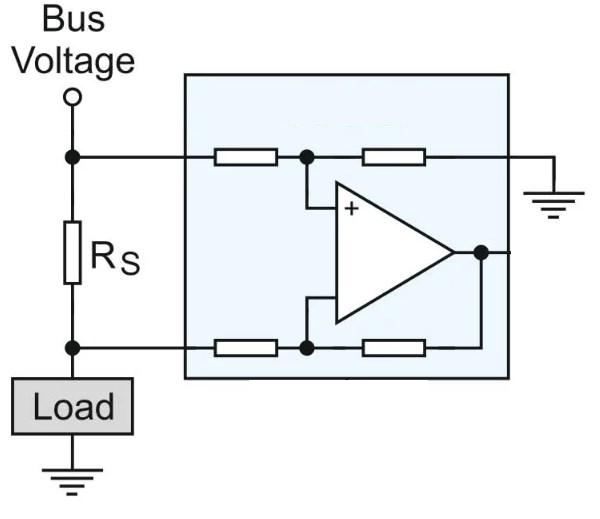
\includegraphics[scale = 0.75]{ris231.png}
  \caption{Схема верхнего плеча}
  \label{ris:231}
\end{figure}

\begin{figure}[H]
  \centering
  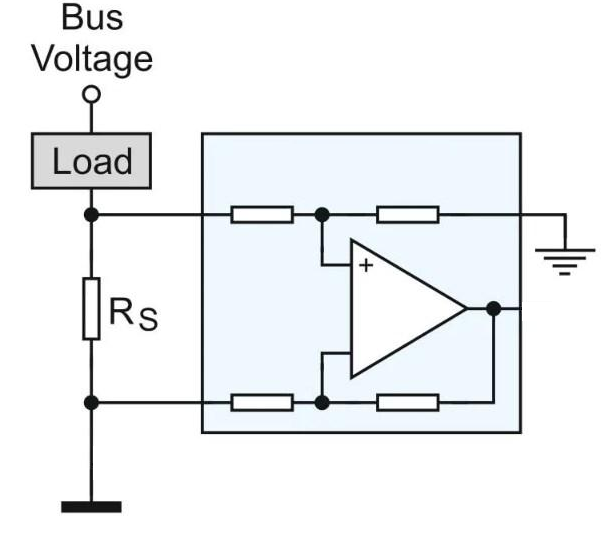
\includegraphics[scale = 0.75]{ris232.png}
  \caption{Схема нижнего плеча}
  \label{ris:232}
\end{figure}

Измерение тока в конфигурации нижнего плеча заключается в размещении измерительного 
элемента между нагрузкой и землей. Этот тип решения довольно легко реализовать, поскольку 
напряжение на измерительном элементе измеряется по отношению к массе цепи. Усилитель 
работает с низкими значениями напряжения (порядка милливольт по отношению к массе схемы), 
что значительно упрощает подбор компонентов и снижает его стоимость.

Основным недостатком этого метода является то, что нагрузка больше не связана напрямую с массой.
 Минусовой вывод нагрузки имеет потенциал на несколько сотен милливольт выше земли, 
 а лучше держать это значение меньше 100 мВ -- эта разница примерно равна падению напряжения
  на шунтирующем резисторе и канале полевого транзистора. Отсутствие прямого соединения
с землей может стать проблемой если в другом месте цепи произойдет короткое замыкание,
    например, если проводящий компонент в устройстве коснется металлического корпуса. 
    Однако для нашего устройства это не будет являться проблемой, так как такой вариант 
    развития событий не предусмотрен.

В случае работы с малыми сигналами довольно большую роль играет входное напряжение 
    смещения усилителя. Чем меньше значение этого параметра, тем выше точность измерения.

Несмотря на эти недостатки, измерение тока на стороне низкого напряжения является хорошим выбором,
 когда нагрузку не нужно подключать напрямую к земле и где нет необходимости обнаруживать 
 короткие замыкания на массу. Но в случае устройств, которые должны соответствовать 
 более строгим требованиям безопасности, измерение тока на стороне высокого 
 напряжения является лучшим выбором.
 После усиления напряжение на выходе ОУ оцифровывается 12-битным АЦП с опорным 
 напряжением 3,3 В, соответственно, каждый значащий разряд АЦП -- это 3,3/4096 = 0,805 мВ.
  При коэффициенте усиления Ку = 50 нашего ОУ, шаг измеряемого напряжения
   на шунте -- около 16 мкВ. Соответственно, при шунтах 100, 1 и 0,01 Ом младшему 
   разряду АЦП соответствует потребляемый ток в 0,16 мкА, 16 мкА и 1,6 мА соответственно 
   \cite{GooglePatent:1}.

\section{Подсистема преобразования уровней}
\hspace{1cm}

Подсистема преобразования уровней нужна для согласования уровней и изоляции от паразитного 
питания шин с разным напряжением. Подсистема будет согласовывать уровни напряжения между
отлдачиком и отлаживаем устройством по линиям передачи данных. 

Надежным и быстрым решением будет использование специализированной микросхемы 74LVC2T45, из-за
следующих преимуществ \cite{SN74LVC2T45:datasheet}:
\begin{itemize}
  \item Работает во всем диапазоне напряжений от 1,65 В до 5,5 В
  \item Имеет функцию изоляции напряжения питания отлаживаемого устройства переводом каналов в
  высокоимпедансное состояние
  \item Малый ток потребления -- до 4 мкА
  \item Минимальная скорость передачи данных 75 Мбит/с
  \item Имеет защиту от статики в соответствии со стандартом JESD20
\end{itemize}
 Ее функциональная диаграмма изображена на рисунке \ref{ris:241}.

\begin{figure}[H]
  \centering
  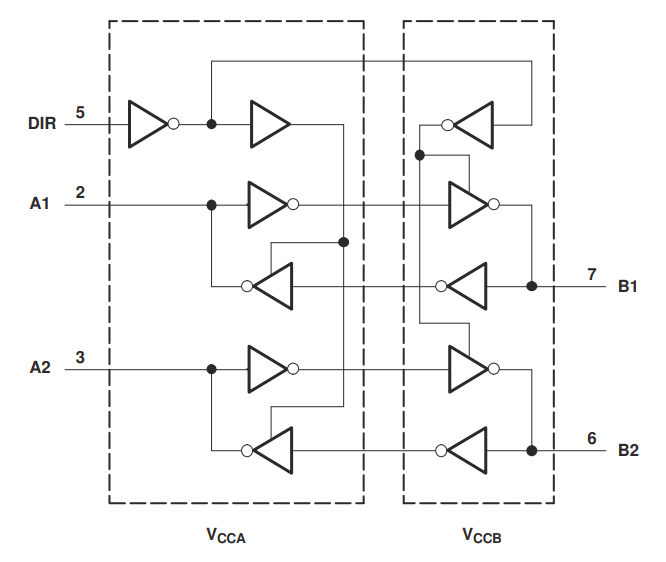
\includegraphics[scale = 0.75]{ris241.png}
  \caption{Функциональная схема 74LVC2T45}
  \label{ris:241}
\end{figure}


\section{Подсистема Ethernet}
\hspace{1cm}

Данная подсистема будет состоять из входного безтрансофрматорного разъема типа RJ-45, 
согласующего трансформатора, и PHY-микросхемы, предназначеной для выполнения функций 
физического уровня сетевой модели OSI.

Связка из безтрансофрматорного разъема и согласующего трансформатора отдельной
микросхмеой была выбрана для совместимости с PoE, так как большинство доступных разъемов со 
встроенным трансмофрматором не имеют отводов от средней точки трансформатора со стороны кабеля,
что необходимо для работы PoE. 

На рисунке \ref{ris:251} изображена внутренняя структура согласующего трансформатора на примере микросхемы
HX1188NL. Проблема у большинства разъемов со встроенным трансформаторо возникала из-за
отсутствия связей 2 и 7. 

\begin{figure}[H]
  \centering
  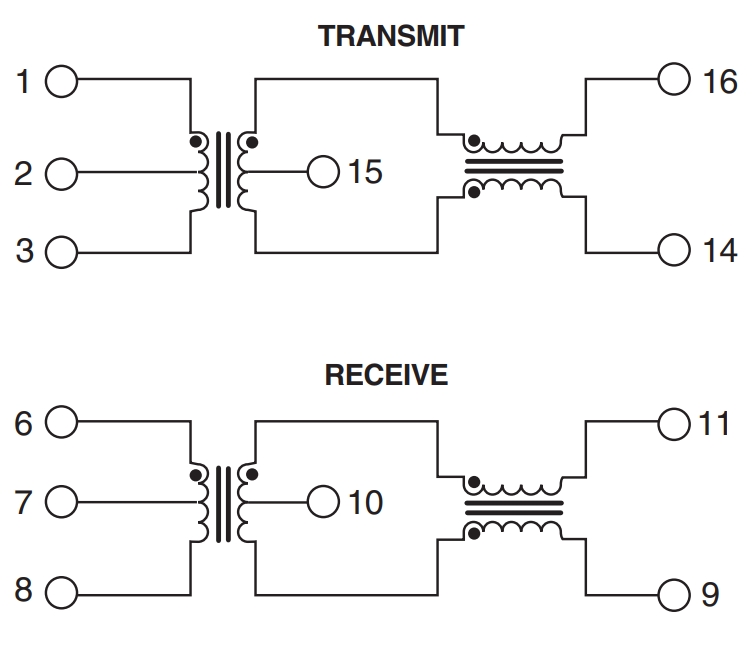
\includegraphics[scale = 0.75]{ris251.png}
  \caption{Внутренняя структура HX1188NL}
  \label{ris:251}
\end{figure}

В качестве Ethernet-контроллера была выбрана микросхема DP83848-EP из-за того, что при отладке
прошивки использовалась отладочная плата именно с этой PHY-микросхемой <<на борту>>. Использование
другой микросхемы привело бы к увелечению времени отладки устройства и более глубокой переработки
уже готового решения, что нерационально.

\section{Структурная схема устройства}
\hspace{1cm}

Исходя из всего вышесказанного, можно составить структурную схему устройства, которая изображена
на рисунке \ref{ris:261}.

\begin{figure}[H]
  \centering
  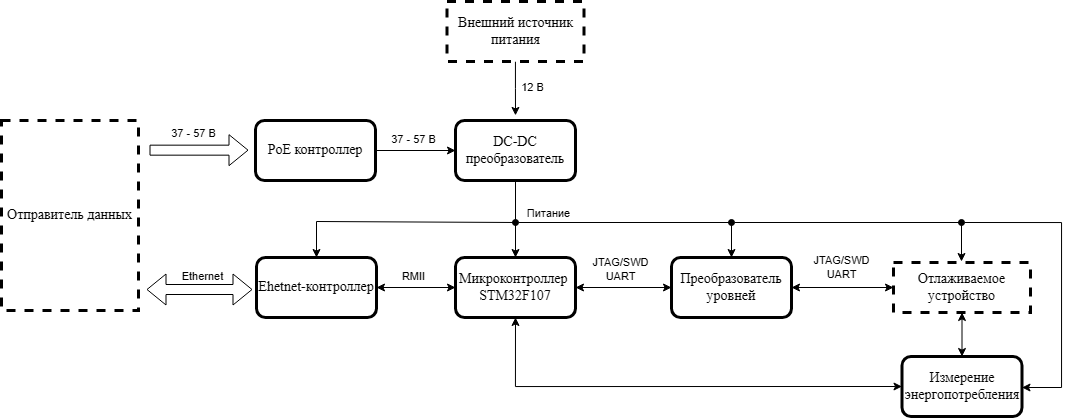
\includegraphics[scale = 0.48]{ris261.png}
  \caption{Структурная схема устройства}
  \label{ris:261}
\end{figure}

Здесь в качестве отправителя выступает условное устройство, от которого будут приходить
команды по Ethernet, PoE-контроллер и DC-DC преобразователь вместе составляют подсистему питания,
Ethernet-контроллер является подсистемой Ethernet, STM32F107 -- подсистема управления, 
преобразователь уровней является подсистемой преобразования уровней, измерение энергопотребления --
это одноименная подсистема, а отлаживаемое устройство представляет собой целевой микроконтроллер,
на который будет отправляться прошивка и чье энергопотребление будет измеряться.

%В случае нехватки объема добавить разгон про модель OSI

%В измерительных приборах вопрос питания стоит особенно остро, ведь даже те помехи, которые 
%не нанесли бы обычному цифровому устройству значительного вреда, могут с легкостью испортить
%всю точность измерения -----------сильная заготовка, но в другую главу-------------
 % описание принципа работы устройства
\begin{thebibliography}{00}

\addcontentsline{toc}{chapter}{Список используемой литературы}

\bibitem{Lakamera:embed} Лакамера, Д.
\emph{Архитектура встраиваемых систем} /Д. Лакамера // ДМК Пресс --
Москва -- 2023. -- 332 с.

\bibitem{STM32:datasheet} Connectivity line, ARM®-based 32-bit MCU with 64/256 KB Flash,
 USB OTG, Ethernet, 10 timers, 2 CANs, 2 ADCs, 14 communication interfaces -- datasheet/
  [Электронный ресурс]
 /STMicroelectronics// -- Март, 2017 -- 
 URL:https://www.st.com/resource/en/datasheet/stm32f107vc.pdf --
 (Дата обращения: 15.05.2024)

\bibitem{TPS2376:datasheet} IEEE 802.3af PoE POWERED DEVICE CONTROLLERS -- datasheet/
  [Электронный ресурс] /Texas Instrument// -- Апрель, 2008 
  -- URL:https://www.ti.com/lit/ds/symlink/tps2376.pdf?ts=1715733862395 --
  (Дата обращения: 15.05.2024)

\bibitem{DP83848:datasheet} DP83848-EP PHYTER™ Military Temperature Single Port
   10/100 Mbps Ethernet
  Physical Layer Transceiver -- datasheet/
  [Электронный ресурс] /Texas Instrument// -- Июнь, 2019 
  -- URL:https://www.ti.com/lit/ds/symlink/dp83848-ep.pdf --
  (Дата обращения: 15.05.2024)

\bibitem{HorHill:ArtOfScheme} Хоровиц, П.
\emph{Искусство схемотехники издание седьмое} /П. Хоровиц, У. Хилл // <<Бином>> --
Москва -- 2003. -- 704 с.

\bibitem{PowerElectronic:FlyBack} Обратноходовой преобразователь /
  [Электронный ресурс] /Алфавит силовой электроники// 
   URL:https://www.power-electronics.info/flyback.html --
  (Дата обращения: 15.05.2024)

\bibitem{GooglePatent:1} M. G. Liberty, “Auto ranging ammeter with accurate measurement 
during range changes. -- URL:
https://patents.google.com/patent/US11774469B2 (Дата обращения: 31.03.2024).

\bibitem{SN74LVC2T45:datasheet} 2-Bit Dual Supply Transceiver with Configurable 
Voltage-Level Shifting and 3-State Outputs
 -- datasheet/
  [Электронный ресурс] /Texas Instrument// -- Октябрь, 2022 -- 
  URL: https://www.ti.com/product/SN74LVC2T45
   --(Дата обращения: 15.05.2024)

\end{thebibliography}
 % ссылки на литературу
\end{document}